\documentclass[11pt]{article}

\usepackage[spanish]{babel}
\usepackage{translations}
\usepackage[titles]{tocloft}
\usepackage{multicol}
\usepackage{graphicx} % Required for the inclusion of images
\usepackage{amsmath} % Required for some math elements 
\usepackage{hyperref}
\usepackage{amsmath}
\usepackage{listings}
\usepackage{courier}
\usepackage[margin=1in]{geometry}
\usepackage{changepage}
\usepackage{titlesec}
\usepackage{wrapfig}
\usepackage[version=4]{mhchem}
\usepackage{multirow}
\usepackage{siunitx}
\usepackage{ragged2e}
\usepackage{adjustbox}
\usepackage[font=small,labelfont=bf]{caption}
\usepackage[table,xcdraw]{xcolor}
\usepackage{afterpage}
\usepackage{xfrac}
\usepackage{animate}
\usepackage{subcaption}
\usepackage{tcolorbox}
\usepackage{nicefrac}

\setlength{\parindent}{1cm}

\definecolor{mytheoremfr}{HTML}{7B0000}
\definecolor{mytheorembg}{HTML}{f5e4e1}

\tcbuselibrary{theorems,skins,hooks}
\newtcbtheorem[number format=\alph]{Theorem}{Pregunta}
{%
	enhanced,
	colback = mytheorembg,
	frame hidden,
	boxrule = 0sp,
	borderline west = {2pt}{0pt}{mytheoremfr},
	sharp corners,
	detach title,
	before upper = \tcbtitle,
	coltitle = mytheoremfr,
	fonttitle = \bfseries\sffamily,
	description font = \mdseries,
	separator sign none,
	segmentation style={solid, mytheoremfr},
}
{th}

\usetikzlibrary{arrows,calc,shadows.blur}
\tcbuselibrary{skins}
\newtcolorbox{note}[1][]{%
	enhanced jigsaw,
	colback=gray!10!white,%
	colframe=gray!80!black,
	size=small,
	boxrule=1pt,
	title=\textbf{Ejercicio:},
	halign title=flush center,
	coltitle=black,
	drop shadow=black!50!white,
	attach boxed title to top left={xshift=1cm,yshift=-\tcboxedtitleheight/2,yshifttext=-\tcboxedtitleheight/2},
	minipage boxed title=2.5cm,
	boxed title style={%
			colback=white,
			size=fbox,
			boxrule=1pt,
			boxsep=2pt,
			underlay={%
					\coordinate (dotA) at ($(interior.west) + (-0.5pt,0)$);
					\coordinate (dotB) at ($(interior.east) + (0.5pt,0)$);
					\begin{scope}[gray!80!black]
						\fill (dotA) circle (2pt);
						\fill (dotB) circle (2pt);
					\end{scope}
				},
		},
	#1,
}

\newcommand{\preguntaAlaMadreDeRocio}[1]{\begin{Theorem}{#1}{}\end{Theorem}}
\newcommand{\laputa}[1]{\begin{note}{#1}{}\end{note}}

\renewcommand{\labelenumi}{\alph{enumi}.} % Make numbering in the enumerate environment by letter rather than number (e.g. section 6)
   
\newcommand{\titulo}{Potenciales en Python\\\ \\(Práctica 1)}
\newcommand{\nombreestudiante}{Víctor Mira Ramírez}
\newcommand{\nombredirector}{J. Fernández-Rossier y Mar Ferri Cortés}
\newcommand{\fecha}{\date{Octubre 2023}}  % Definir solo el año de presentación

\pagebreak

\renewcommand{\listtablename}{Índice de tablas} 
\renewcommand{\tablename}{Tabla} 
\renewcommand\cftsecdotsep{\cftdotsep}

\setlength{\cftbeforesecskip}{0.5ex}
\renewcommand{\cftsecfont}{%
  \fontsize{11}{13}\usefont{OT1}{phv}{bc}{n}\selectfont
}
\makeatletter
\renewcommand{\@pnumwidth}{1.75em}
\renewcommand{\@tocrmarg}{2.75em}
\makeatother

\begin{document}

\begin{titlepage}
	\centering
	
\includegraphics[width=65mm]{fotos/logoUA.png}\par
	\vspace{1cm}
	{\huge\bfseries \vspace{15mm} \titulo \par}
	\vfill
	{\large 
	\vfill
	Estudiante:\par\vspace{2mm}
	\nombreestudiante\par
	\vfill
	Profesor:\par\vspace{2mm}
    \nombredirector
    \vfill
    Universidad de Alicante\par
    Facultad de Ciencias: Departamento de Física Aplicada\par
    Mecánica Cuántica 1\par
	\fecha\par}
\end{titlepage}

\pagebreak

\begin{abstract}\label{sec:abstract}
    \noindent El objetivo de esta práctica es aprender a resolver la ecuación de Schrödinger en una dimensión para potenciales arbitrarios de forma numérica usando \textit{Python}. Para ello se estudiaran dos problemas propuestos y se discutirá brevemente la física que les concierne: el efecto túnel y túnel resonante, así como los estados ligados de potenciales en una dimensión.
\end{abstract}

\tableofcontents

\section*{Introducción}
    \noindent Práctica realizada durante el curso 23-24 para la asignatura de Mecánica Cuántica I de la Universidad de Alicante. Clases de prácticas impartidas por J. Fernández-Rossier y Mar Ferri Cortés. Mi DNI es 74528754Z, cuyas tres últimas cifras son 754, que será relevante para las cuestiones que se discuten más adelante.\\
    
    \noindent Es importante para el funcionamiento adecuado de los códigos proporcionados en este informe se cambie el nombre del archivo proporcionado en clase a 'PRAC12023.py', ya que el que viene por defecto al descargarlo no puede ser leído directamente por \textit{python}. A lo largo del informe usamos como valores iniciales: $xmax=50$, $m=1$, $N=150$.
    
\section{Primer Problema (Modelo 1)}
    
    \subsection{Apartado A}
    \laputa{Encuentre el valor de la diferencia de energía, $\Delta \equiv E_1 - E_0$, para $p = 0$. (Observa que esta cantidad dependerá ligeramente de los valores de \textit{N} y \textit{xmax} elegidos para los cálculos).}

        \noindent El primer paso es definir nuestra función de potencial, que siguiendo los parámentros del guión y mi DNI será:
        \begin{equation}
            V(x)=\dfrac{p}{2}x^2-10x
        \end{equation}
        \noindent Ahora, nos haremos valer de la función \textit{ham} proporcionada, así como de la función \textit{eigh} de la librería \textit{scipy.linalg} para crear una función \textit{DeltaRespectoP} que nos devuelva la diferencia de energía entre el estado $E0$ y el estado $E1$ proporcionando un $p$ a la función.\\
    
        \noindent Ejecutando \textit{DeltaRespectoP(0)} obtenemos el valor deseado, que aparece impreso por consola una vez ejecutado.    
        \begin{equation}
            \Delta \equiv E_1 - E_0 = 126.697\ meV \hspace{1.5cm}\text{para }p=0
        \end{equation}

    \subsection{Apartado B}
    \laputa{Encuentra el valor del parámetro \textit{p} en el potencial $V(x)$ que te corresponde, tal que el cambio de diferencia de energía entre el estado fundamental $E_0$ y el primer excitado es $E_1$ con respecto al obtenido en el apartado anterior, $\Delta(p) - \Delta(0)$, sea igual tres últimas cifras de tu DNI en $meV$. Por ejemplo, DNI terminado en $437$, $\Delta(p) - \Delta(0)=437meV$.}

        \noindent Para la resolución de este apartado crearemos una función \textit{BuscaP} que se hará valer de la función del apartado anterior \textit{DeltaRespectoP} para encontrar el valor de $p$ que haga que $\Delta(p) - \Delta(0)= 745\ meV$\\
        \begin{equation}
            p = 75.641\ \pm 0.009\ \nicefrac{meV}{A^2}
        \end{equation}
        
    \subsection{Apartados C y D}
    \laputa{\textbf{(FIGURA 1)} Dibuja la curva $\Delta(p) - \Delta(0)$ como función del parámetro variable de tu potencial, y haz visible la solución del problema en dicho punto.}
    \laputa{\textbf{(FIGURA 2)} Dibuja las funciones de onda de los estados para 
    el valor \textit{p} obtenido.}  

        \noindent Nos hacemos valer del valor de $p$ obtenido en el apartado anterior así como de la función \textit{plotstates} del código de la práctica.
        \begin{figure}[ht]
            \centering
            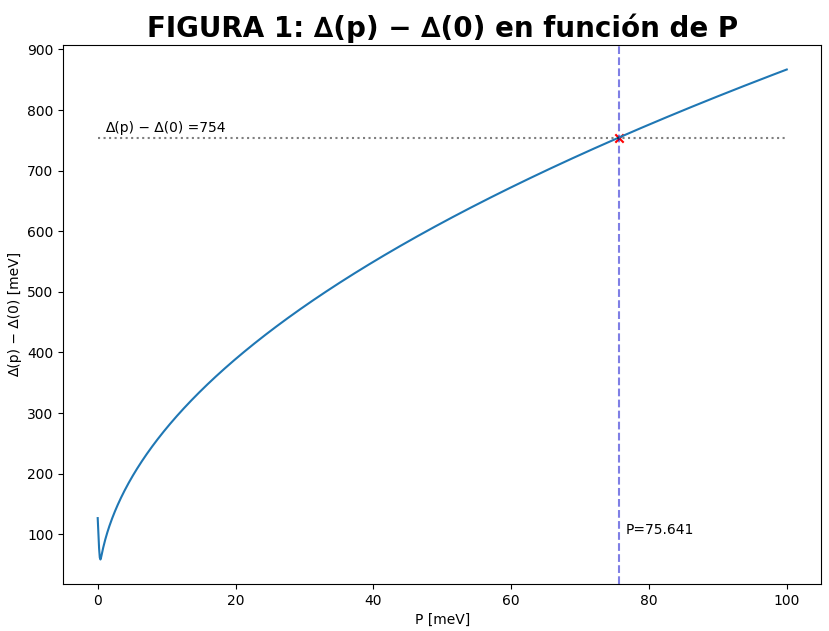
\includegraphics[width=0.46\textwidth]{fotos/Figure_1.png}
            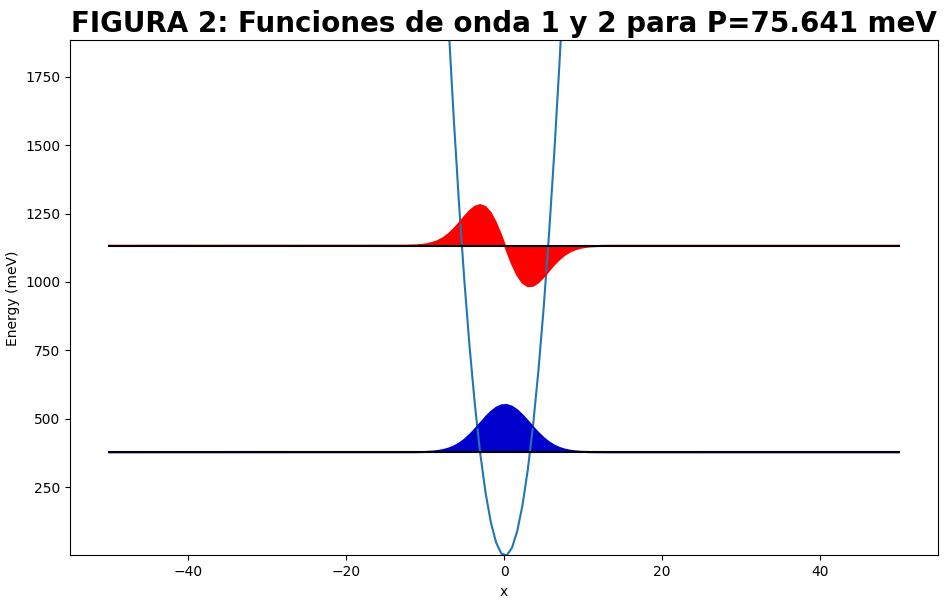
\includegraphics[width=0.53\textwidth]{fotos/Figure_2.png}
        \end{figure} 

\clearpage
\section{Segundo Problema (Modelo 2)}
    \subsection{Apartados A y B}
    \laputa{Determina la energía del electrón para que la probabilidad de transmisión $T$ sea igual a las $3$ últimas cifras de tu DNI, divididas por $1000$ (Por ejemplo, para $DNI = 63290281, T = 0.281$). Nota que puede haber más de una energía que satisface la condición requerida.}
    \laputa{\textbf{(FIGURA 3)} Grafica la curva $T(E)$ correspondiente en la que se vea la solución del apartado anterior.}

    \begin{wrapfigure}[13]{r}{0.55\textwidth}
        \vspace{-0.6cm}
        \centering
        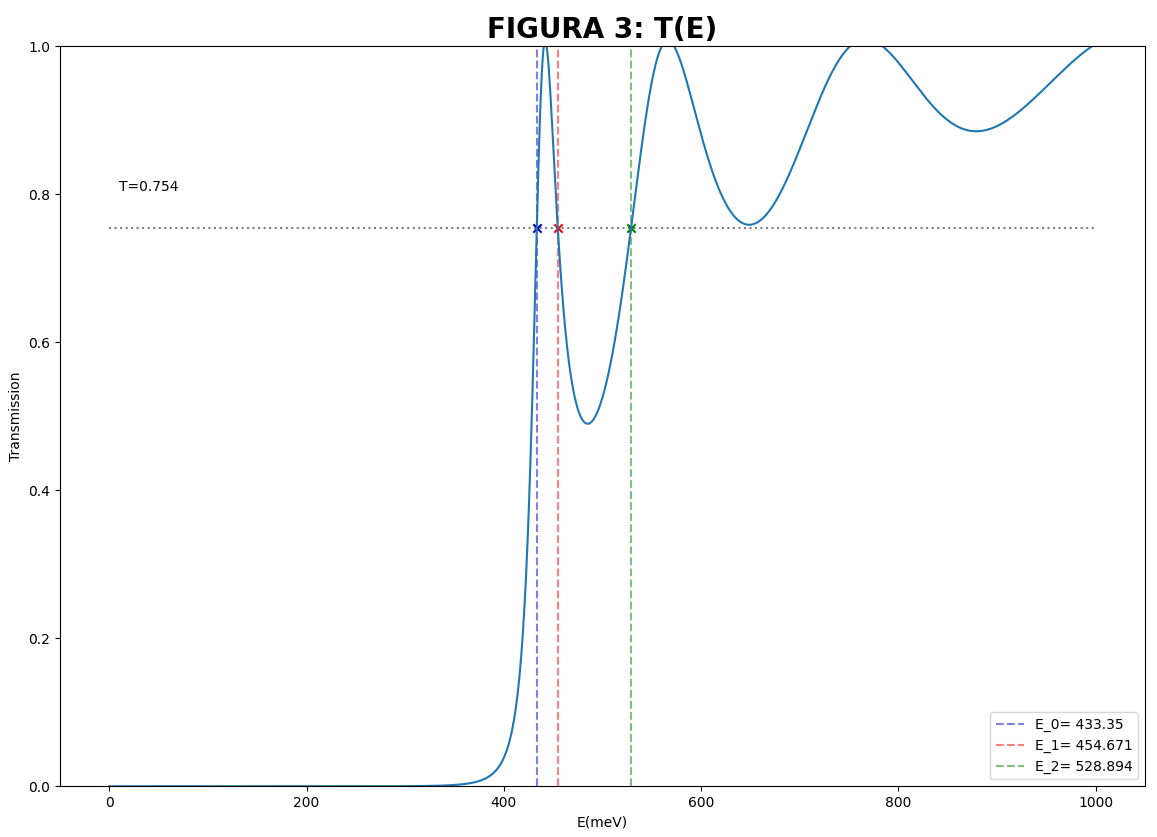
\includegraphics[width=0.53\textwidth]{fotos/Figure_3.png}
    \end{wrapfigure} 

    \noindent Como en el problema anterior, lo primero que hacemos es definir nuestra función de potencial, haciendo uso de \textit{doublebarrier} del código de la práctica. Ahora, crearemos una función \textit{buscaE} que dada una transmisión objetivo y una precisión, calcula para qué energía (o energías) se da dicha precisión.\\

    \noindent La función va calculando la transmisión haciendo uso de la función \textit{trans} proporcionada por el guión de la práctica, y cuando la diferencia entre la transmisión calculada y la objetivo es menor a una tolerancia (por defecto de $10^{-4}$) guarda dicho valor en una lista. Este método hace que para un mismo punto de corte podamos tener múltiples valores de energía que cumplan la condición de tolerancia, por lo que nos quedamos con el que menor error genere.\\

    \noindent Finalmente el programa imprime por consola los valores de las energías que cumplen que $T=0.754$:
    \begin{equation}
        E_0 = 433.350\ meV \hspace{2cm} E_1 = 454.671\ meV \hspace{2cm} E_2 = 528.894\ meV
    \end{equation}

    \noindent Haremos uso de la función \textit{plotT} para graficar la transmisión, añadiendo los datos obtenidos y obteniendo la figura deseada. Puede parecer debido a la baja resolución que hay un cuarto corte en la figura, pero con suficiente precisión no se da el caso.

\section{Anexos}
    \subsubsection*{Hipervínculo al código de python que hace los cálculos y genera las gráficas:}
        \href{https://github.com/vmr48-ua/extras/blob/main/MC1-P1.py}{MC1-P1.py}
    \subsubsection*{Hipervínculo al código de LaTeX que genera este documento:}
        \href{https://www.overleaf.com/read/dfygzrrhtvtd#b13bac}{MC1 - Práctica 1: Potenciales en Python.tex}
    
\end{document} 